\chapter{ESTADO DEL ARTE}\label{cap:estado-arte}
\listasdecapitulo{2}

El estado del arte se organiza en torno a los cinco subsistemas que estructuran la solución propuesta: el
sensado y la detección vehicular, el control adaptativo, la arquitectura de cómputo en el borde y la nube
con sus comunicaciones, la ciberseguridad y confiabilidad, y la validación por simulación. Cada sección
revisa de forma crítica las tecnologías disponibles, las contrasta en una tabla comparativa y concluye con
el criterio adoptado para el diseño, de modo que la revisión bibliográfica justifique directamente las
decisiones que se desarrollan en los capítulos siguientes.

\section{Sensado y detección vehicular}\label{sec:sensado}

Todo esquema de semaforización inteligente se sostiene sobre dos pilares: medir con fiabilidad la demanda
vehicular y actuar las señales con eficiencia. Durante décadas la solución dominante fue el lazo inductivo. Se trata de una espira de conductor alojada bajo
el asfalto que actúa como un sensor de inductancia: el chasis metálico de un vehículo detenido sobre la espira
altera su valor, y ese cambio se traduce en una señal de presencia (Buchanan, 2023). El método es preciso y
prácticamente inmediato, pero paga esas virtudes con una instalación intrusiva —hay que cortar la carpeta
asfáltica— y con un deterioro que reaparece en cada repavimentación.

En la última década se han incorporado sensores sobre la superficie para complementar o reemplazar a los
lazos. Las cámaras de vídeo permiten una detección flexible (múltiples carriles, peatones y clasificación de
tipos de vehículo) y sirven además para vigilancia de infracciones; su desempeño puede degradarse con
condiciones climáticas adversas (humedad y polvo, frecuentes en Lima) o iluminación deficiente, y requieren
algoritmos de visión artificial para interpretar la imagen. Los radares de microondas, instalados sobre el
semáforo, miden el reflejo de las ondas para detectar vehículos y estimar su velocidad, operan de día y de
noche y bajo lluvia, pero su costo es elevado. Los magnetómetros inalámbricos detectan los cambios en el
campo magnético terrestre producidos por los vehículos y, al conectarse en red, facilitan la instalación sin
cableado y la cobertura modular de varios puntos de la intersección (Gheorghe y Soica, 2025).

\begin{figure}[H]
  \centering
  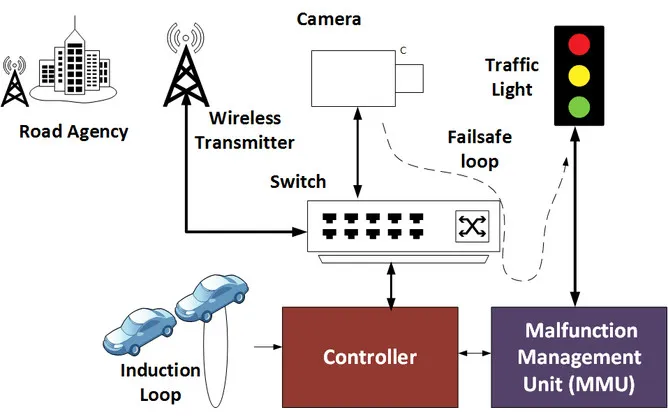
\includegraphics[width=0.8\linewidth,keepaspectratio]{media/image25.png}
  \caption{Vista general de un sistema de control de tráfico con detección en la vía.}
  \label{fig:sistema-trafico}
  \fuente{Buchanan (2023).}
\end{figure}

En el lado de la actuación, las ópticas semafóricas migraron al LED. Frente a la lámpara incandescente, el LED
consume una fracción de la energía —del orden de una quinta parte—, se mantiene operativo durante decenas de
miles de horas y ofrece una indicación más contrastada; a ello se añade que, al integrarse cada bombillo con
varios diodos, la avería de uno no apaga la señal, lo que aporta redundancia (Buchanan, 2023). La etapa que
gobierna estas luces está sujeta a requisitos que impiden combinaciones peligrosas, y por eso el gabinete
aloja una unidad de gestión de fallos (\emph{Malfunction Management Unit}, MMU) que, ante cualquier
inconsistencia en la secuencia de luces, obliga al cruce a pasar a intermitencia ámbar como estado seguro
(Buchanan, 2023). A estos
elementos se suman los dispositivos de demanda peatonal (pulsadores o sensores de presencia) que informan al
controlador la necesidad de servir la fase peatonal.

\subsection{Métodos de visión por computadora para detección vehicular}

Cuando la fuente de detección es la cámara, la información visual debe procesarse para extraer conteo,
clasificación, velocidad y longitud de cola. Aun con recursos de cómputo escasos, los enfoques clásicos de sustracción de fondo siguen prestando servicio.
El modelo de mezcla de gaussianas (MOG2) representa la intensidad de cada píxel mediante varias gaussianas que
se adaptan a los cambios lentos de luz, y ofrece buena precisión en escenas urbanas estables (Zivkovic, 2004).
El descriptor de gradientes orientados HOG (\emph{Histogram of Oriented Gradients}) es eficaz para localizar
peatones en el cruce, aunque pierde fiabilidad ante las oclusiones frecuentes cuando la intersección se satura
(Dalal y Triggs, 2005). Los clasificadores en cascada de Haar, muy ligeros, permiten estimar la velocidad con
poco error al combinarse con un seguidor, a cambio de una mayor tasa de falsos positivos (Viola y Jones, 2001).

Con la irrupción del aprendizaje profundo, estas técnicas cedieron el protagonismo a los detectores
neuronales de tiempo real. Los modelos de la familia YOLO (\emph{You Only Look Once}) abordan en un solo paso
la ubicación y el tipo de cada objeto de la escena, y ese diseño de una sola pasada es el que les permite
conservar buena exactitud a las cadencias de cuadro que exige el tráfico; de ahí su difusión para el conteo y
la clasificación de vehículos en vídeo (Redmon et al., 2016). Como la detección se realiza fotograma a
fotograma, se acompaña de un seguidor que preserva la identidad de cada vehículo en el tiempo: Deep SORT
(\emph{Simple Online and Realtime Tracking with Deep Association Metric}) añade, a la trayectoria estimada por
un filtro de Kalman, un descriptor de apariencia calculado por una red neuronal, y ese rasgo visual reduce de
forma sustancial los cruces de identidad propios de un seguimiento puramente cinemático (Wojke et al., 2017).
Detección y seguimiento, en conjunto, son los que permiten derivar flujo, cola y velocidad a partir de una
sola cámara. La selección concreta de la arquitectura de detección y de la
plataforma de cómputo corresponde al diseño electrónico y se aborda en los capítulos posteriores; aquí
interesa establecer que la visión por computadora es técnicamente madura para sustituir o complementar a los
sensores empotrados.

\begin{table}[H]
  \centering
  \caption{Comparativa de tecnologías de detección vehicular en intersecciones.}
  \label{tab:sensado}
  \begin{tabularx}{\linewidth}{@{}>{\raggedright\arraybackslash}p{0.18\linewidth}XX>{\raggedright\arraybackslash}X@{}}
    \toprule
    \textbf{Tecnología} & \textbf{Principio} & \textbf{Ventajas} & \textbf{Limitaciones} \\
    \midrule
    Lazo inductivo & Variación de inductancia al paso del vehículo & Alta precisión, respuesta inmediata & Instalación invasiva, mantenimiento costoso \\
    Cámara + visión & Procesamiento de imagen (detección y seguimiento) & Cobertura amplia, clasificación y métricas múltiples por carril & Sensible a clima e iluminación, requiere cómputo dedicado \\
    Radar de microondas & Reflexión de microondas en el vehículo & Opera de día/noche y con mal clima, mide velocidad & Costo elevado, cobertura focal \\
    Magnetómetro inalámbrico & Perturbación del campo magnético terrestre & Instalación sencilla, malla flexible & Alcance limitado, vida de batería finita \\
    \bottomrule
  \end{tabularx}
  \fuente{Elaboración propia.}
\end{table}

\textbf{Criterio adoptado.} La comparación de la Tabla~\ref{tab:sensado} justifica adoptar la cámara con
visión por computadora como fuente principal de detección: es la única tecnología que provee de forma
simultánea conteo, clasificación, velocidad y cola con una instalación no invasiva, aprovechable sobre la
infraestructura existente. Sus limitaciones ante condiciones adversas se mitigan con sensores auxiliares de
diagnóstico y con un actuado fiable basado en LED y mecanismos de \emph{failsafe} (MMU), de modo que el
sensado se equilibre entre costo, facilidad de despliegue e interoperabilidad.

\section{Control adaptativo}\label{sec:control}

El controlador de tráfico es la unidad lógica que recibe la información de los sensores y ejecuta la
temporización de las luces. Las estrategias de control adaptativo se revisan a continuación en orden de
creciente autonomía y dependencia de datos —control clásico analítico, heurísticas de optimización en línea,
lógica difusa y aprendizaje por refuerzo—, de modo que la comparación justifique el núcleo de control
adoptado. Los esquemas convencionales operan con planes de tiempo fijo o con control
actuado, en el que cada fase se activa ante la demanda detectada y la duración de verde se extiende hasta un
máximo predefinido mientras persistan vehículos. La formulación de Webster (1958) fue la primera en dar una
regla analítica de temporización: dedujo el ciclo que minimiza la demora total, $C_0 = (1{,}5L + 5)/(1 - Y)$,
donde $L$ agrupa el tiempo perdido por ciclo e $Y$ suma las razones de flujo crítico de las fases. La expresión
es útil mientras la intersección opera con holgura, pero pierde fiabilidad cuando el grado de saturación se
aproxima a la unidad: el denominador $1-Y$ tiende a cero, el ciclo calculado se dispara y las duraciones
dejan de ser realistas (Webster, 1958). El refinamiento de Akçelik (1981) amplió este marco analítico con una
fórmula de demora dependiente del tiempo, aplicable también en régimen de sobresaturación donde la
formulación original pierde precisión. El valor de esta familia clásica reside en su interpretabilidad y
simplicidad analítica para intersecciones aisladas, a costa de no reaccionar a la fluctuación de la demanda
dentro del ciclo.

Sobre ese cimiento surgieron los sistemas adaptativos comerciales. SCATS (\emph{Sydney Coordinated Adaptive
Traffic System}) ajusta, ciclo a ciclo, la duración total y el reparto de verdes según el grado de saturación
que registran los detectores en la línea de parada (Fehon, 2016); SCOOT (\emph{Split Cycle Offset Optimization
Technique}) se apoya en detectores situados aguas arriba y aplica correcciones pequeñas y continuas al reparto
y a los desfases para enlazar olas verdes sucesivas. Ambos son de gobierno centralizado y consiguen reducir la
demora y ampliar la capacidad, a cambio de una calibración cuidadosa y de una inversión considerable en
instrumentación y comunicaciones. Como alternativa descentralizada, Surtrac (\emph{Scalable Urban Traffic Control}) hace que
cada intersección decida localmente de forma asíncrona y comunique a sus vecinas una proyección de su flujo
de salida, lo que mejora la escalabilidad y la robustez ante fallos de comunicación; logró reducciones
significativas de tiempos de viaje en pruebas de campo en Pittsburgh (Smith, Barlow, Xie y Rubinstein, 2013).
En el Perú, los controladores instalados manejan hasta 20 fases y pueden coordinar varias intersecciones; el
distrito de San Isidro implementó el controlador ITC-3 de SWARCO, modular y compatible con TCP/IP y NTCIP,
enlazado a un centro de control distrital (ITS Perú, 2024).

\begin{figure}[H]
  \centering
  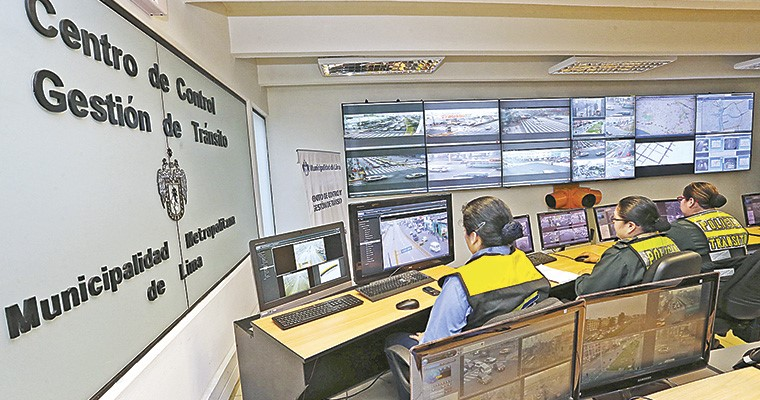
\includegraphics[width=0.8\linewidth,keepaspectratio]{media/image17.png}
  \caption{Centro de control de gestión de tránsito de la Municipalidad Metropolitana de Lima.}
  \label{fig:centro-control}
  \fuente{ITS Perú (2024).}
\end{figure}

Más allá de los sistemas comerciales cíclicos, las heurísticas analíticas de optimización en línea constituyen
una familia descentralizada que prescinde de un ciclo fijo y decide la fase a servir a partir del estado
instantáneo de las colas. El control por máxima presión (\emph{Max-Pressure}), formalizado por Varaiya (2013),
evalúa en cada instante la \emph{presión} de cada fase —la diferencia entre lo acumulado en los enlaces de
entrada y en los de salida— y sirve aquella que más reduce ese desbalance; al resolver cada cruce por su
cuenta, la política es descentralizada y cuenta con una garantía teórica de que las colas permanecen acotadas.
Un principio afín guía a las estrategias autoorganizadas SOTL (\emph{Self-Organizing Traffic Lights}), que
conmutan la fase según umbrales de acumulación vehicular. La evidencia comparativa resulta ilustrativa para situar el resto de
técnicas: en un marco abierto sobre SUMO con 32 semillas aleatorias, Max-Pressure igualó o superó a
controladores de aprendizaje profundo (DQN, DDPG) en tiempo de viaje, con una reducción cercana al 25\,\%
frente al control de tiempo fijo (Genders y Razavi, 2019). Que una heurística simple alcance al aprendizaje
profundo matiza la necesidad de recurrir a modelos de caja negra y motiva el uso de controladores
interpretables como la lógica difusa.

\subsection{Lógica difusa como núcleo del control adaptativo}

Entre las técnicas de aprendizaje aplicadas al control de tráfico, la lógica difusa destaca por combinar un
desempeño elevado con interpretabilidad. Un controlador difuso convierte cantidades medidas en grados de
pertenencia a etiquetas cualitativas —\emph{tráfico pesado}, \emph{cola larga}, \emph{espera excesiva}—
mediante funciones de membresía, y combina un conjunto de reglas \emph{si--entonces} para decidir si prolongar
o cambiar la fase. Reproduce así la manera en que un ingeniero de tránsito razona sobre el cruce y, a
diferencia de un modelo de caja negra, mantiene cada regla explícita y por tanto inspeccionable, verificable y
certificable antes de su puesta en marcha; esa transparencia resulta decisiva en un esquema donde la autoridad
última de seguridad sigue recayendo en el controlador.

En términos de desempeño, la evidencia reportada es favorable: el control difuso alcanza una mejora cercana
al 74\,\% respecto de los controladores de tiempo fijo, superando a Q-learning (66\,\%) y a redes neuronales
simples (71\,\%), y el proyecto europeo FUSICO lo validó como método especialmente efectivo en condiciones
de tráfico irregular (Koukol et al., 2015). El método de Mamdani resulta más adecuado para intensidades
bajas y medias, y se han documentado reducciones de los tiempos de espera de alrededor del 35\,\% frente a
estrategias convencionales en casos de estudio reales.

De manera más específica, dos trabajos del mismo grupo de investigación aportan validaciones cuantitativas
directamente comparables con la solución propuesta, al combinar un sistema difuso de Mamdani con el cálculo de
ciclo de Webster sobre SUMO. Ali et al. (2021) afinan fase a fase, mediante defuzzificación por centroide, el
verde estimado por la fórmula de Webster aplicada en tiempo real, y reportan reducciones del tiempo de espera
de hasta 41,7\,\% con datos reales de campo y de 49,4\,\% bajo demanda variable frente al Webster de tiempo
fijo, con la observación de que la ventaja del control adaptativo se maximiza cuando la demanda fluctúa en el
tiempo. Yalcinli et al. (2024) modelan a escala 1:1 una intersección real en SUMO y, con un esquema adaptativo
de extensión de fase por densidad, obtienen 27,2\,\% menos demora, 32,4\,\% menos tiempo de espera y 16,7\,\%
más velocidad respecto del tiempo fijo, valores que verifican de forma cruzada contra la fórmula de Webster y
contra una medición por cámara, lo que enlaza la validación en simulación con la detección por visión. Esta
combinación de mejora cuantificable, interpretabilidad y validabilidad fundamenta la elección de la lógica
difusa de Mamdani como núcleo del control adaptativo de la solución propuesta.

El aprendizaje por refuerzo profundo (DRL) cierra esta progresión como contrapunto: aprende políticas
mediante interacción continua con el entorno y alcanza mejoras competitivas en redes complejas, pero a costa
de requisitos que comprometen su uso en operación crítica. Rafique et al. (2024) muestran que su agente
necesita 300 episodios de entrenamiento para converger y que el desempeño puede degradarse fuera del régimen
aprendido: la variante \emph{turn-based} empeora hasta 67\,\% en alta demanda, mientras que la variante
\emph{time-based}, más conservadora, alcanza alrededor del 35\,\% de mejora promedio sobre el tiempo fijo. A
ello se suma la marcada sensibilidad a los hiperparámetros documentada por Genders y Razavi (2019), quienes
observan que los métodos con más hiperparámetros (SOTL, DQN, DDPG) presentan una varianza notablemente mayor
y deben optimizarse antes de cualquier comparación, pues un ajuste deficiente puede inducir conclusiones
erróneas. Esta fragilidad, unida a la baja interpretabilidad que dificulta certificar cada decisión, justifica
por contraste la elección de un control difuso de Mamdani: no requiere entrenamiento, no es frágil ante
cambios de régimen y resulta trazable y validable regla a regla. Por ello el DRL se reserva como capa
experimental de optimización global, sin sustituir al control difuso local validable.

Los órdenes de magnitud reportados por la literatura cuantitativa de control adaptativo se resumen en la
Tabla~\ref{tab:resultados-adaptativo}, que sirve de referencia para situar el desempeño esperable del núcleo
difuso propuesto frente a líneas base clásicas, heurísticas y de aprendizaje por refuerzo.

\begin{table}[H]
  \centering
  \caption{Resultados reportados por la literatura de control adaptativo.}
  \label{tab:resultados-adaptativo}
  \begin{tabularx}{\linewidth}{@{}>{\raggedright\arraybackslash}p{0.12\linewidth}>{\raggedright\arraybackslash}X>{\raggedright\arraybackslash}X>{\raggedright\arraybackslash}p{0.11\linewidth}>{\raggedright\arraybackslash}X@{}}
    \toprule
    \textbf{Trabajo (año)} & \textbf{Controladores} & \textbf{Simulador / escenario} & \textbf{Métrica principal} & \textbf{Mejora reportada vs.\ fijo} \\
    \midrule
    Genders y Razavi (2019) & Tiempo fijo, Webster, Max-Pressure, SOTL, DQN, DDPG & SUMO; dos intersecciones; 32 semillas aleatorias & Tiempo de viaje & Max-Pressure: $\sim$25\,\% menos (59 frente a 79\,s); iguala o supera al RL profundo \\
    Ali et al. (2021) & Webster fijo, Webster modificado, Difuso+Webster, Difuso+Webster modificado, difuso puro & SUMO+TraCI; intersecciones reales de 3/4/5 ramas (Kilis) & Tiempo de espera & Difuso+Webster: 41,7\,\% menos (datos reales) y 49,4\,\% menos (demanda variable) \\
    Yalcinli et al. (2024) & Tiempo fijo frente a modelo adaptativo (ablación de tres componentes) & SUMO; intersección real de Heybe (Antalya), hora pico & Demora por vehículo & 27,2\,\% menos demora; 32,4\,\% menos espera; 16,7\,\% más velocidad \\
    Rafique et al. (2024) & RL \emph{turn-based} y \emph{time-based} frente a tiempo fijo & SUMO; una intersección de 4 ramas; demanda Low/High/EW/NS & Tiempo de espera acumulado & \emph{Time-based}: $\sim$35\,\% en promedio (hasta 57\,\% en alta demanda); \emph{turn-based} se degrada (hasta 67\,\% peor) \\
    \bottomrule
  \end{tabularx}
  \fuente{Elaboración propia a partir de las fuentes citadas.}
\end{table}

\begin{table}[H]
  \centering
  \caption{Comparativa de estrategias de control semafórico.}
  \label{tab:control}
  \begin{tabularx}{\linewidth}{@{}>{\raggedright\arraybackslash}p{0.12\linewidth}XX>{\raggedright\arraybackslash}p{0.13\linewidth}>{\raggedright\arraybackslash}p{0.12\linewidth}>{\raggedright\arraybackslash}p{0.12\linewidth}@{}}
    \toprule
    \textbf{Controlador} & \textbf{Principio} & \textbf{Datos requeridos} & \textbf{Interpre\-tabilidad} & \textbf{Escala\-bilidad} & \textbf{Mejora reportada} \\
    \midrule
    Webster & Cálculo analítico del ciclo óptimo & Flujos de saturación por acceso & Alta & Aislada & 10--15\,\% \\
    SCATS & Ajuste cíclico centralizado por saturación & Detectores en línea de parada & Media & Media & 12--20\,\% \\
    SCOOT & Optimización incremental de desfases & Detectores aguas arriba & Media & Media & $\sim$12\,\% \\
    Surtrac & Programación distribuida multiagente & Colas y tiempos de llegada & Media & Muy alta & $\sim$25\,\% \\
    Difuso & Reglas lingüísticas si--entonces & Flujo, cola y espera locales & Alta & Media & $\sim$74\,\% \\
    DRL & Política aprendida por refuerzo & Gran volumen de datos/entrenamiento & Baja & Alta & 27--68\,\% (experimental) \\
    \bottomrule
  \end{tabularx}
  \fuente{Elaboración propia a partir de las fuentes citadas en la sección.}
\end{table}

\textbf{Criterio adoptado.} La Tabla~\ref{tab:control} muestra que, frente a controladores de mayor mejora
nominal pero baja interpretabilidad (DRL) o de gran dependencia de infraestructura centralizada (SCATS,
SCOOT), la lógica difusa ofrece el mejor equilibrio entre mejora reportada, interpretabilidad y validabilidad
local. Se adopta, por tanto, un control difuso que opera de forma autónoma en cada intersección como
herramienta de recomendación, mientras el controlador semafórico existente conserva la autoridad final y las
funciones críticas de seguridad; la coordinación global y el DRL se reservan como capas de optimización
futura.

El núcleo difuso de esta tesis se inscribe explícitamente en la familia difuso+Webster validada por Ali et
al. (2021) y Yalcinli et al. (2024): un sistema de Mamdani interpretable que afina en tiempo real el verde
calculado por la fórmula de ciclo óptimo, sin requerir entrenamiento previo ni comprometer la trazabilidad de
cada decisión. Su validación se desarrolla en el Capítulo~\ref{cap:validacion}, donde el controlador propuesto
se compara contra líneas base clásicas (tiempo fijo y Webster) y heurísticas (control actuado y máxima
presión) bajo escenarios reproducibles y semillas aleatorias.

\section{Arquitectura edge--nube y comunicaciones}\label{sec:arquitectura}

Incorporar la Internet de las Cosas (IoT) al control semafórico aporta conectividad y operación remota. En
concreto, dota a cada controlador de un módulo capaz de observar su entorno, comunicarse y dejarse administrar
desde la nube: remite en tiempo real conteos, estados y fallos hacia servidores que ejecutan analítica
intensiva y conservan el histórico, y recibe de vuelta parámetros o recomendaciones ya validados.

El punto delicado de esa integración es la latencia cuando la decisión debe tomarse al instante. Delegar cada
ciclo a un servidor remoto y aguardar su respuesta pondría en riesgo la reacción del semáforo; para evitarlo
se recurre al cómputo en el borde (\emph{edge computing}), que resuelve localmente, en el propio módulo de la
intersección, la lógica que fija el ciclo, y reserva para la nube las tareas de mayor alcance —coordinar
intersecciones, optimizar a escala de red y supervisar— (Gheorghe y Soica, 2025). Con este reparto el cruce
sigue funcionando con seguridad aun sin enlace, y aprovecha la conexión, cuando existe, para afinar su
desempeño con información global.

\begin{figure}[H]
  \centering
  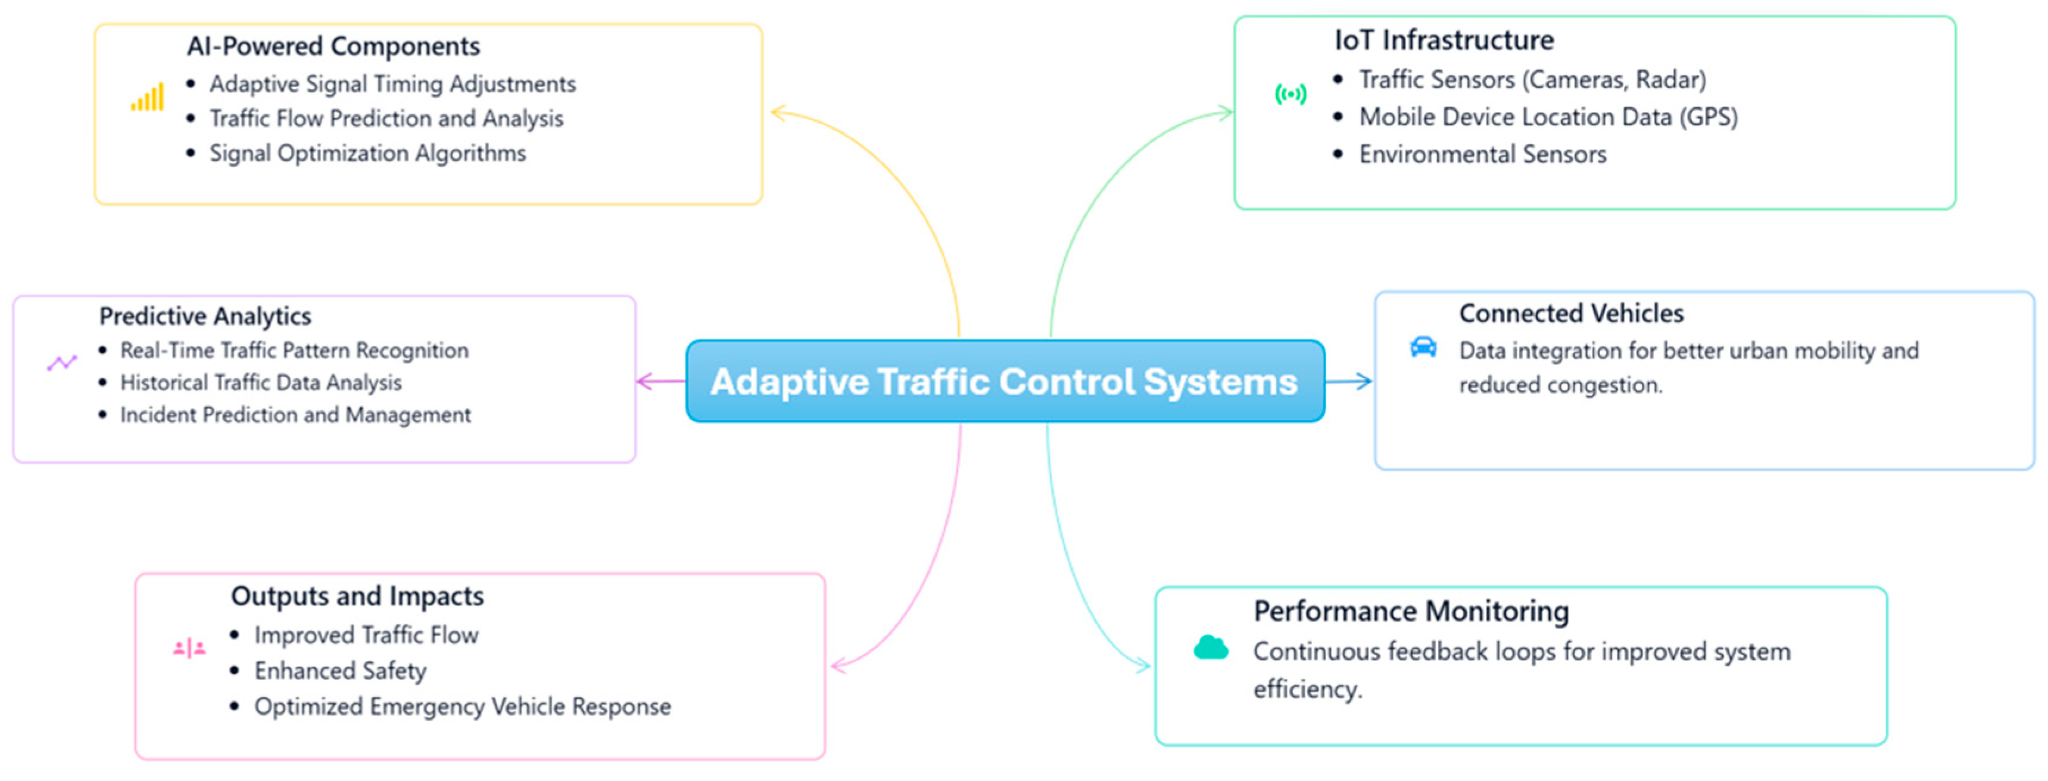
\includegraphics[width=0.8\linewidth,keepaspectratio]{media/image82.png}
  \caption{Componentes funcionales de un sistema de control de tráfico adaptativo basado en IoT.}
  \label{fig:componentes-iot}
  \fuente{Gheorghe y Soica (2025).}
\end{figure}

La interoperabilidad entre componentes descansa en los protocolos de comunicación. NTCIP (\emph{National
Transportation Communications for ITS Protocol}) es el marco de referencia para el diálogo entre los equipos
de campo y los centros de gestión: organizado en capas, permite que dispositivos de distintos fabricantes se
entiendan y atiende solicitudes de prioridad con retardos por debajo de medio segundo; su perfil para
controladores de señales actuadas (NTCIP 1202) goza de amplio soporte en los equipos actuales (NTCIP, 2025).
La telemetría del lado IoT se cursa con MQTT (\emph{Message Queuing Telemetry Transport}): su esquema de
publicación y suscripción y su encabezado reducido lo hacen apropiado para transmitir lecturas de sensores con
alta frecuencia de actualización y entrega fiable sobre redes urbanas (Banks y Gupta, 2014). Por encima de ambos, TCP/IP actúa como capa de transporte de red
común a los equipos, la central y los servicios remotos. La separación de roles entre estos protocolos evita
presentar a la nube como reemplazo del controlador certificado y preserva una jerarquía segura de decisión,
como se resume en la Tabla~\ref{tab:protocolos}.

\begin{table}[H]
  \centering
  \caption{Rol de los protocolos principales en la arquitectura propuesta.}
  \label{tab:protocolos}
  \begin{tabularx}{\linewidth}{@{}>{\raggedright\arraybackslash}p{0.18\linewidth}XX>{\raggedright\arraybackslash}X@{}}
    \toprule
    \textbf{Protocolo / capa} & \textbf{Uso dentro del sistema} & \textbf{Tipo de información} & \textbf{Criterio de seguridad} \\
    \midrule
    TCP/IP & Capa base de comunicación entre equipos de red, central, módulo IoT y servicios remotos. & Paquetes de datos, transporte de mensajes y servicios de red. & Segmentación de red, filtrado por firewall y monitoreo de disponibilidad. \\
    NTCIP & Interoperabilidad con el controlador semafórico y la central de gestión. & Estados de operación, configuración de fases y parámetros permitidos por el controlador. & Uso restringido al dominio semafórico y validación por el controlador existente. \\
    MQTT sobre TLS & Telemetría del módulo IoT hacia la nube y recepción de recomendaciones o parámetros. & Métricas de tráfico, alarmas, estado energético, eventos y datos agregados. & Autenticación por certificados, cifrado TLS y control de tópicos autorizados. \\
    Interfaz de operador & Supervisión local/remota desde la central semafórica. & Visualización, alertas, reportes y aprobación de acciones críticas. & RBAC, MFA, registro de auditoría y separación entre monitoreo y mando. \\
    \bottomrule
  \end{tabularx}
  \fuente{Elaboración propia.}
\end{table}

\textbf{Criterio adoptado.} Se adopta una arquitectura híbrida borde--nube en la que el módulo IoT actúa como
puente seguro entre el nivel local y la nube: habilita decisiones locales inmediatas y, a la vez, envía
información agregada para la optimización global. La pila de comunicaciones se acota a NTCIP para la
interoperabilidad con el controlador, MQTT sobre TLS para la telemetría IoT y TCP/IP como transporte, de modo
que la arquitectura sea escalable y tolerante a fallos: el semáforo opera con seguridad incluso sin enlace a
la nube.

\section{Ciberseguridad y confiabilidad}\label{sec:ciberseguridad-arte}

La interconexión de los semáforos con la nube y otros dispositivos, que en su origen fueron equipos aislados,
los expone a riesgos cibernéticos capaces de afectar la operación urbana: manipulación de la señalización,
inyección de datos falsos o acceso no autorizado al control de tránsito. Un caso documentado en los Países
Bajos demostró que era posible manipular remotamente semáforos IoT enviando datos falsos de bicicletas
inexistentes para forzar el cambio de luces, debido a la ausencia de autenticación robusta en la comunicación
(Kirk, 2020; Buchanan, 2023). La ciberseguridad es, por tanto, un requisito de diseño y no un añadido.

Las defensas se organizan en capas complementarias. El cifrado de extremo a extremo sobre TLS/SSL protege la
confidencialidad y la integridad de los datos mientras viajan y habilita que los dispositivos se autentiquen
entre sí. La autenticación multifactor (MFA) y el control de acceso por roles (RBAC) limitan quién ingresa y
qué puede hacer cada uno una vez dentro. Las firmas digitales acreditan el origen y la integridad de cada
mensaje; las redes privadas virtuales (VPN) y los cortafuegos separan el tráfico legítimo de las amenazas
externas. Por último, revisar las vulnerabilidades de forma periódica y aplicar los parches sin dilación
mantiene la protección al día frente a ataques nuevos.

\begin{table}[H]
  \centering
  \caption{Mecanismos de ciberseguridad para semáforos inteligentes IoT.}
  \label{tab:ciberseg-mecanismos}
  \begin{tabularx}{\linewidth}{@{}>{\raggedright\arraybackslash}p{0.22\linewidth}XX>{\raggedright\arraybackslash}X@{}}
    \toprule
    \textbf{Mecanismo} & \textbf{Ventajas} & \textbf{Limitaciones} & \textbf{Uso en semáforos inteligentes} \\
    \midrule
    Cifrado de extremo a extremo (E2EE) & Confidencialidad de los datos de principio a fin. & Puede aumentar la latencia por cifrado/descifrado. & Protege las comunicaciones entre los semáforos y la nube. \\
    Protocolos de transporte (TLS/SSL) & Protege las comunicaciones en tránsito y su integridad. & Requiere gestión correcta de certificados. & Asegura las conexiones entre dispositivos IoT y la nube. \\
    Autenticación multifactor (MFA) & Refuerza la seguridad con múltiples capas de verificación. & Añade pasos de acceso para los operadores. & Garantiza que solo personal autorizado acceda a los controles. \\
    Firmas digitales & Verifica autenticidad e impide modificaciones no autorizadas. & Requiere infraestructura de gestión de claves. & Asegura el origen verificado de los datos enviados a la nube. \\
    VPN y firewalls & Aíslan la red semafórica de amenazas externas. & Demandan inversión y mantenimiento adicionales. & Protegen los semáforos y la nube de accesos no autorizados. \\
    RBAC & Gestiona el acceso a las funciones según el rol. & Complejo de administrar con muchos usuarios. & Asigna niveles de acceso adecuados a cada operador. \\
    Análisis de vulnerabilidades & Identifica debilidades antes de su explotación. & Exige monitoreo y actualización constantes. & Mantiene la seguridad en el tiempo mediante parches. \\
    \bottomrule
  \end{tabularx}
  \fuente{Elaboración propia.}
\end{table}

Para que la seguridad no quede como una mera lista de mecanismos, se plantea un modelo de amenazas aplicado a
la arquitectura propuesta. Este modelo identifica los puntos de exposición más relevantes y define
mitigaciones coherentes con un módulo IoT que complementa al controlador semafórico, sin sustituir sus
funciones críticas de seguridad funcional.

\begin{table}[H]
  \centering
  \caption{Modelo de amenazas del sistema IoT semafórico.}
  \label{tab:amenazas-arte}
  \begin{tabularx}{\linewidth}{@{}>{\raggedright\arraybackslash}p{0.20\linewidth}XX>{\raggedright\arraybackslash}X@{}}
    \toprule
    \textbf{Amenaza} & \textbf{Impacto posible} & \textbf{Punto vulnerable} & \textbf{Mitigación propuesta} \\
    \midrule
    Suplantación del módulo IoT & Ingreso de telemetría falsa o recomendaciones no autorizadas. & Conexión MQTT y registro de dispositivos. & Certificados por dispositivo, lista blanca, rotación de credenciales y revocación. \\
    Manipulación de datos de tráfico & Optimización basada en información incorrecta. & Telemetría, API externa y datos de visión. & Validación cruzada, límites físicos, detección de valores anómalos y auditoría. \\
    Acceso no autorizado de operador & Modificación indebida de parámetros o consulta de datos sensibles. & Interfaz de monitoreo y consola administrativa. & MFA, RBAC, registros de auditoría y separación entre roles de lectura y mando. \\
    Denegación de servicio & Pérdida temporal de conexión con la nube o la central. & Enlace de comunicación y broker MQTT. & Operación local degradada, almacenamiento temporal, reintento controlado y alertas. \\
    Compromiso físico del gabinete & Daño de sensores, corte de energía o manipulación de interfaces. & Gabinete, cableado y periféricos externos. & Gabinete IP65/IK, cerradura, sensores de apertura y procedimientos de mantenimiento. \\
    \bottomrule
  \end{tabularx}
  \fuente{Elaboración propia.}
\end{table}

La arquitectura debe diferenciar la ciberseguridad de la seguridad funcional. La ciberseguridad protege la
información y el acceso al sistema; la seguridad funcional evita estados semafóricos peligrosos incluso ante
una falla de software, de comunicación o de energía. Por ello, el módulo IoT se plantea como capa de sensado,
análisis y recomendación, mientras que el controlador semafórico mantiene la autoridad final sobre la
ejecución segura de las fases, según los criterios de la Tabla~\ref{tab:seg-funcional}.

\begin{table}[H]
  \centering
  \caption{Criterios de seguridad funcional para el módulo propuesto.}
  \label{tab:seg-funcional}
  \begin{tabularx}{\linewidth}{@{}>{\raggedright\arraybackslash}p{0.26\linewidth}XX@{}}
    \toprule
    \textbf{Condición} & \textbf{Respuesta requerida} & \textbf{Justificación} \\
    \midrule
    Pérdida de comunicación con la nube & El controlador mantiene el plan local vigente y el módulo IoT almacena datos hasta recuperar conexión. & Evita depender de la nube para decisiones críticas en tiempo real. \\
    Datos anómalos o inconsistentes & Se descartan recomendaciones fuera de límites y se genera una alerta de diagnóstico. & Reduce el riesgo de actuar sobre mediciones erróneas o manipuladas. \\
    Falla del módulo IoT & El controlador semafórico continúa operando con su lógica convencional. & Conserva la continuidad del servicio aunque falle la capa adaptativa. \\
    Solicitud de ola verde prioritaria & La sugerencia debe respetar tiempos mínimos, conflictos de fases y la validación del controlador. & Evita generar condiciones inseguras para peatones y flujos transversales. \\
    \bottomrule
  \end{tabularx}
  \fuente{Elaboración propia.}
\end{table}

\textbf{Criterio adoptado.} El diseño aplica una defensa por capas (cifrado TLS, MFA, RBAC, firmas digitales,
segmentación y auditoría) acompañada de un modo degradado seguro. El principio rector es la separación entre
recomendación y actuación: el módulo IoT puede ser comprometido o quedar incomunicado sin que ello derive en
un estado semafórico peligroso, porque el controlador certificado conserva la autoridad final.

\section{Validación por simulación}\label{sec:validacion}

La simulación por computadora permite probar estrategias y tecnologías de control en un entorno controlado
antes de su implementación real. Los simuladores de tráfico varían en su nivel de detalle y capacidad de
integración con sistemas externos, criterio decisivo para validar un controlador adaptativo en lazo cerrado.

PTV VISSIM es un microsimulador comercial de gran detalle y fidelidad, dotado de una interfaz 3D potente, que
representa uno a uno vehículos y peatones y admite control adaptativo a través de APIs externas y módulos
V2X; se le reconoce como referente en calibración fina, si bien su licencia es cara y reclama hardware
exigente (Bedoya Reyes, 2013). AIMSUN adopta un enfoque híbrido micro-mesoscópico: tan pronto sigue cada
vehículo como lo agrupa en flujos para aligerar el cálculo en redes amplias; acepta planes reales de SCATS o
SCOOT y permite ensayar algoritmos por su API, a costa de una calibración más experta (Bedoya Reyes, 2013).
Synchro 8, apoyado en el motor del \emph{Highway Capacity Manual} 2010, se orienta al análisis y la
optimización de intersecciones y se acopla a SimTraffic para la simulación, con un perfil más analítico que
de control en tiempo real (Trafficware, 2014).

SUMO (\emph{Simulation of Urban Mobility}) es un microsimulador de código abierto, muy arraigado en la
investigación y capaz de crecer hasta redes de gran tamaño. A su gratuidad y amplia configurabilidad añade la
interfaz TraCI (\emph{Traffic Control Interface}), que mantiene abierto un canal con la simulación en
ejecución: un proceso externo —por ejemplo, el propio módulo de control IoT— consulta el estado del tráfico e
introduce acciones, como forzar el cambio de una indicación, sin detener la corrida. Esa posibilidad de
intervenir en marcha es la que lo vuelve idóneo para ensayar controladores adaptativos en lazo cerrado;
además importa mapas reales desde OpenStreetMap y simula comunicaciones entre vehículos, si bien exige una
calibración manual atenta para reproducir las condiciones reales. Por estas características, SUMO es el microsimulador de
código abierto más utilizado para desarrollar y evaluar algoritmos de control semafórico antes de su
despliegue en campo, como evidencian los trabajos de referencia en control adaptativo (Ali et al., 2021;
Genders y Razavi, 2019); además, habilita una comparación reproducible mediante semillas aleatorias y líneas
base comunes, condición necesaria para contrastar el controlador propuesto con estrategias clásicas y
heurísticas en igualdad de condiciones.

\begin{figure}[H]
  \centering
  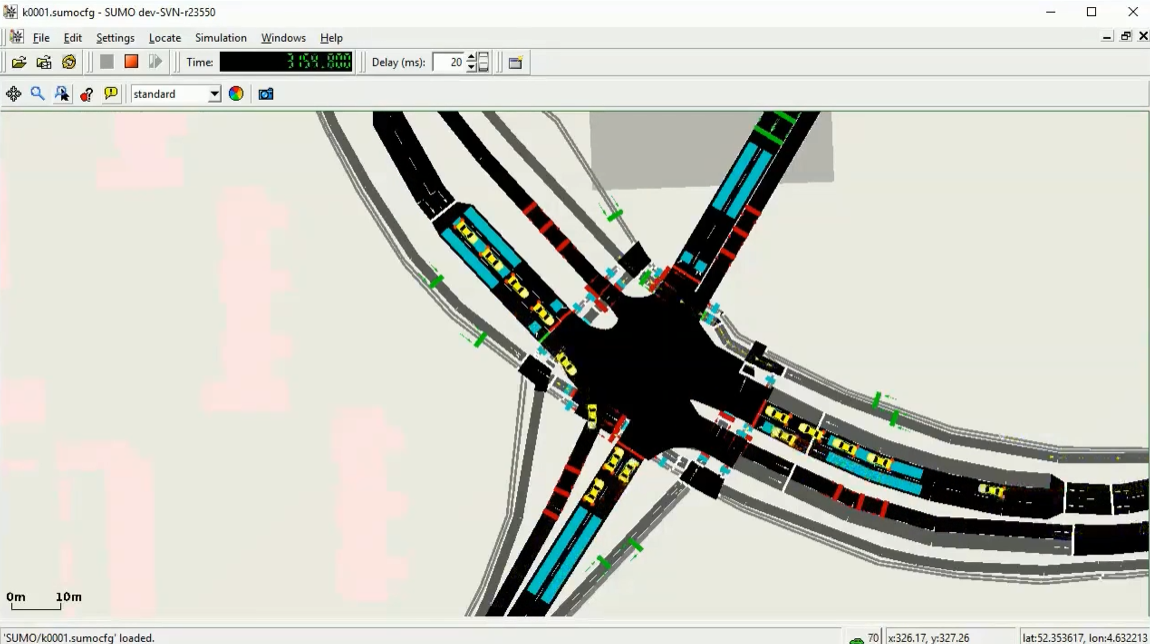
\includegraphics[width=0.8\linewidth,keepaspectratio]{media/image144.png}
  \caption{Interfaz del simulador de tráfico de código abierto SUMO.}
  \label{fig:sumo}
  \fuente{Elaboración propia.}
\end{figure}

\begin{table}[H]
  \centering
  \caption{Comparativa de simuladores de tráfico.}
  \label{tab:simuladores}
  \begin{tabularx}{\linewidth}{@{}>{\raggedright\arraybackslash}p{0.15\linewidth}>{\raggedright\arraybackslash}p{0.20\linewidth}XX@{}}
    \toprule
    \textbf{Simulador} & \textbf{Tipo} & \textbf{Características principales} & \textbf{Integración con sistemas externos} \\
    \midrule
    PTV VISSIM & Microscópico (comercial) & Alta fidelidad, visualización 3D, semáforos programables, V2X. & APIs externas; costo de licencia elevado. \\
    AIMSUN & Híbrido micro-mesoscópico & Planes SCATS/SCOOT, vehículos autónomos, optimización en tiempo real. & API para algoritmos; mayor exigencia de calibración. \\
    SUMO & Microscópico (código abierto) & Gratuito, escalable, mapas reales, comunicaciones vehiculares. & TraCI: comunicación en vivo y control en lazo cerrado. \\
    Synchro 8 & Análisis/mesoscópico & Optimización de intersecciones, motor HCM 2010, SimTraffic. & Integración con otros simuladores (UTDF). \\
    \bottomrule
  \end{tabularx}
  \fuente{Elaboración propia.}
\end{table}

\textbf{Criterio adoptado.} La comparación de la Tabla~\ref{tab:simuladores} sustenta la elección de SUMO con
TraCI para la validación: su carácter abierto y la comunicación en vivo permiten conectar el controlador
adaptativo externo, reproducir escenarios y evaluar métricas de cola, espera, velocidad y congestión, además
de emular condiciones de comunicación y ciberseguridad. VISSIM o AIMSUN podrían reservarse para validaciones
puntuales de micro-detalle o presentación visual a interesados.

Para cerrar el estado del arte, la Tabla~\ref{tab:sintesis} integra las lecciones extraídas de cada
subsistema con el criterio adoptado y su aplicación en la solución propuesta, evidenciando la trazabilidad
entre la revisión bibliográfica y las decisiones de diseño desarrolladas en los capítulos siguientes.

\begin{table}[H]
  \centering
  \caption{Síntesis del estado del arte y criterios adoptados para la solución propuesta.}
  \label{tab:sintesis}
  \begin{tabularx}{\linewidth}{@{}>{\raggedright\arraybackslash}p{0.16\linewidth}XX>{\raggedright\arraybackslash}X@{}}
    \toprule
    \textbf{Eje tecnológico} & \textbf{Lección del estado del arte} & \textbf{Criterio adoptado} & \textbf{Aplicación en la tesis} \\
    \midrule
    Sensado vehicular & La visión por computadora aporta flujo, colas y clasificación, aunque requiere calibración y respaldo ante condiciones adversas. & Usar la cámara como fuente principal y sensores auxiliares para diagnóstico. & Módulo IoT con cámara, sensores ambientales y monitoreo energético. \\
    Control adaptativo & El control difuso combina mejora cuantificable con interpretabilidad y validabilidad. & Priorizar el control difuso local validable y dejar la optimización global como recomendación. & Control local autónomo, coordinación por nube y validación en simulación. \\
    Comunicaciones & La interoperabilidad exige separar los protocolos industriales de la telemetría IoT. & NTCIP para el entorno semafórico y MQTT/TLS para la telemetría. & Arquitectura compatible con el controlador existente y servicios en la nube. \\
    Ciberseguridad & Los sistemas conectados requieren autenticación, cifrado y trazabilidad. & Diseñar defensa por capas y modo degradado seguro. & TLS, MFA, RBAC, auditoría y controlador como autoridad final. \\
    Validación & La simulación permite comparar estrategias antes de intervenir la infraestructura real. & Usar SUMO/TraCI para escenarios reproducibles. & Evaluación de métricas de cola, espera, velocidad y congestión. \\
    \bottomrule
  \end{tabularx}
  \fuente{Elaboración propia.}
\end{table}
